\chapter{Trabalhos Correlatos}

O objetivo desta seção é realizar uma análise comparativa de aplicações que apresentam um contexto similar ao do presente TCC. Para isso, faremos uma descrição sucinta de cada trabalho correlato, seguida de uma comparação dos requisitos que são comumente oferecidos por todas essas aplicações. A intenção é explorar as similaridades e as diferenças entre elas para aprimorar nosso entendimento e guiar o desenvolvimento do nosso projeto.

\section{ValidaWeb: Uma ferramenta para suporte ao desenvolvimento de software atendendo aos requisitos não funcionais de acessibilidade W3C}

O ValidaWeb \cite{validaweb}, é uma ferramenta voltada ao suporte no desenvolvimento de software voltados para a Web, que valida estruturas HTML e CSS com o objetivo de retornar sugestões sobre possíveis melhorias voltadas a acessibilidade. Tem como base os requisitos da W3C para definição de quais as propriedades são necessárias para uma boa acessibilidade do software que está sendo desenvolvido.

\begin{figure}[!h]
	\centering
	\caption{Tela Principal do VSCode com a extensão ValidWeb.}
	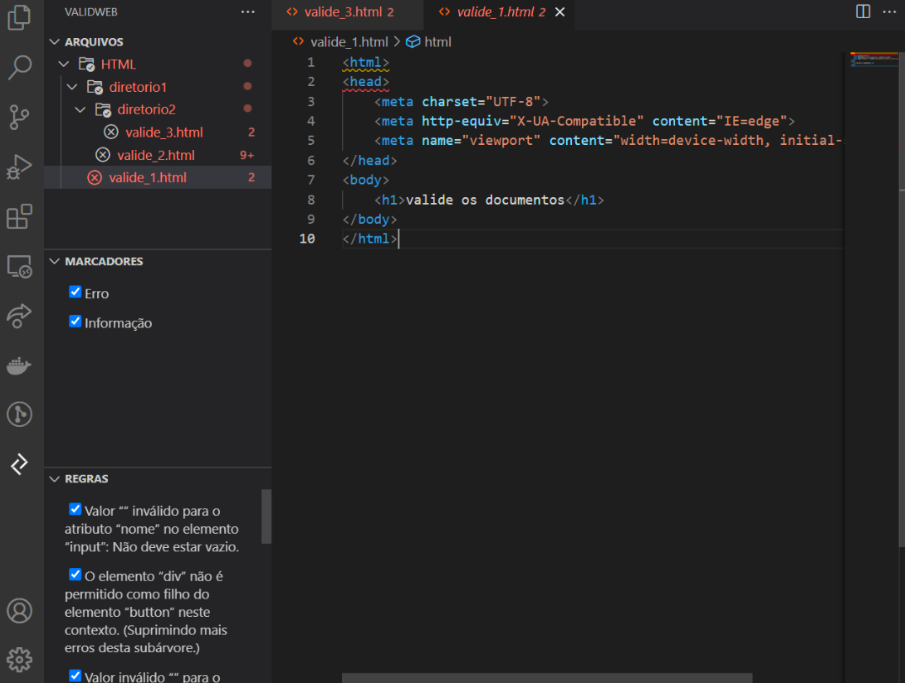
\includegraphics[width=432pt]{Assets/ValidaWeb.png}
	\fonte{\cite[p. 59]{validaweb}}
\end{figure}

A interface proposta pelo ValidWeb é intuitiva e prática. Por meio de destaques no texto, os desenvolvedores são notificados sobre inconsistências nas especificações de acessibilidade, que devem ser resolvidas para que esses destaques sejam removidos. Além disso, a ferramenta de \cite{validaweb} também permite a geração de relatórios em PDF do estado atual do código, facilitando sua análise e compartilhamento com outros desenvolvedores, especialmente em ambientes de desenvolvimento que envolvem múltiplas equipes com controle de qualidade rigoroso.

Dessa forma, o ValidWeb e o presente TCC compartilham objetivos similares, embora tenham focos tecnológicos distintos.

\section{SonarQube: Ferramenta de auditoria de código com suporte para Flutter e Dart}

O SonarQube, conforme descrito pela \cite{sonarqube}, é uma ferramenta robusta de análise estática de código. Seu objetivo é simplificar a padronização de projetos para desenvolvedores. A ferramenta dispõe de uma interface gráfica intuitiva que destaca os principais pontos de atenção na qualidade estática do código. Dentre os indicadores apresentados estão: número de bugs, vulnerabilidades, "Security Hotspots", dívida técnica, "Code Smells", cobertura de testes e linhas de código duplicadas, conforme ilustrado na Figura 4.

\begin{figure}[!h]
	\centering
	\caption{Interface principal do SonarQube.}
	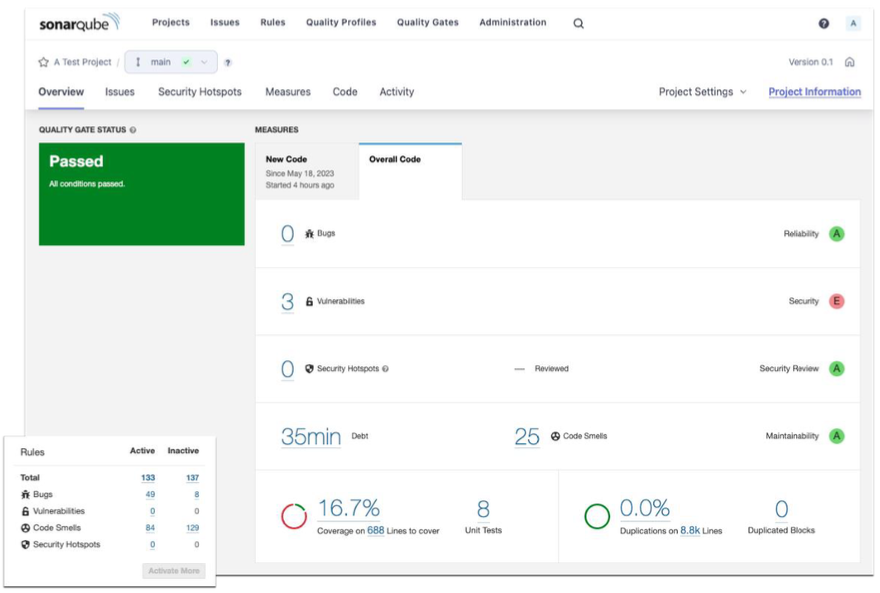
\includegraphics[width=432pt]{Assets/SonarQube.png}
	\fonte{\cite{sonarflutter}}
\end{figure}

Por padrão, a ferramenta não oferece suporte para a linguagem Dart e o framework Flutter. No entanto, graças ao esforço da comunidade, especificamente da InsideApp \cite{sonarflutter}, uma empresa focada no desenvolvimento de aplicações móveis, foi criado um plugin que permite a interoperabilidade básica entre Flutter, Dart e SonarQube. Este plugin aproveita as regras padrões estabelecidas pelo Flutter para realizar a análise e fornecer sugestões de melhorias.

Ainda que o foco principal do SonarQube não seja a acessibilidade, a ferramenta, em conjunto com o SonarLint - também desenvolvido pela SonarSource \cite{sonarqube} - oferece sugestões ao desenvolvedor durante o processo de codificação na IDE. Esta funcionalidade se assemelha à proposta do presente TCC, demonstrando a potencialidade de uso dessas ferramentas em conjunto para melhorar tanto a qualidade do código quanto sua acessibilidade.

\section{accessibility\_tools: Pacote para validação de acessibilidade em aplicações Flutter}

Conforme descrito pela Rebel AppStudio, mantenedora do pacote, o accessibility\_tools é uma suíte de ferramentas destinadas a melhorar a acessibilidade em aplicações desenvolvidas com Flutter. \cite{accessibilitytools} destaca a importância da acessibilidade em aplicativos, ressaltando que "Criar um aplicativo acessível é extremamente importante. No entanto, é comum esquecer ou adiar essas melhorias. Este pacote garante que seu aplicativo seja acessível desde o primeiro dia, verificando a interface logo que é construída".

A Figura 5 exemplifica o funcionamento da ferramenta durante a fase de desenvolvimento de uma aplicação. A ferramenta opera em tempo de execução, enfatizando possíveis melhorias de acessibilidade por meio de mensagens exibidas diretamente na interface.

\begin{figure}[!h]
	\centering
	\caption{Exemplo de retorno do pacote “accessibility\_tools” ao detectar uma inconsistência de acessibilidade.}
	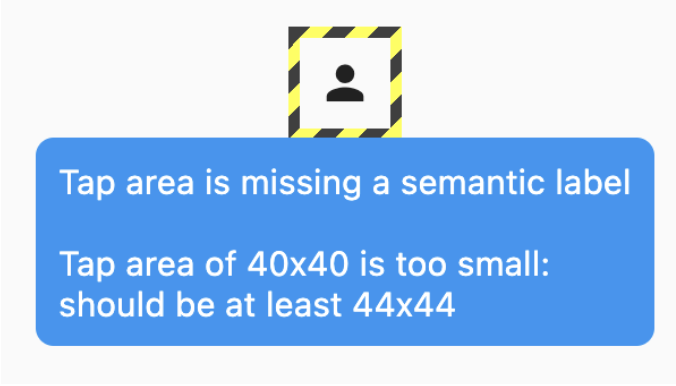
\includegraphics[width=384pt]{Assets/AccessibilityTools.png}
	\fonte{\cite{accessibilitytools}}
\end{figure}

Até agosto de 2023, o pacote suporta a validação de áreas mínimas de toque, semântica de botões, sobreposição de textos e descrição de campos de entrada. Embora a ferramenta cubra apenas alguns aspectos de acessibilidade, ela representa um ponto de partida valioso para desenvolvedores Flutter interessados em melhorar a acessibilidade de suas aplicações.

A abordagem adotada no presente TCC difere em aspectos importantes. Em vez de operar em tempo de execução, o foco está na análise estática de código para fornecer sugestões diretamente na IDE. Isso elimina a necessidade de compilar e executar a aplicação para avaliar as necessidades de acessibilidade, permitindo que os desenvolvedores identifiquem e resolvam problemas de acessibilidade mais rapidamente.

\section{Análise e comparação de trabalhos correlatos}

O universo de ferramentas disponíveis para auxiliar no desenvolvimento de aplicações acessíveis é vasto e diversificado. No entanto, as ferramentas discutidas neste capítulo foram escolhidas por sua relevância e semelhanças com a proposta deste TCC. Cada uma delas utiliza um conjunto de regras ou requisitos não funcionais de acessibilidade para estabelecer padrões e oferecer sugestões de modificações, dependendo do estado da aplicação em desenvolvimento. A identificação desses requisitos será uma etapa crucial na elaboração da proposta deste TCC.

Na Tabela 1 a seguir, é feita uma comparação entre as funcionalidades das ferramentas discutidas e os requisitos deste trabalho. Esta tabela ajuda a identificar áreas para melhoria na proposta deste TCC e também destaca as deficiências das outras ferramentas em comparação com a proposta atual.

\begin{table}[!h]
	\centering
	\caption{Comparação entre as funcionalidades das ferramentas discutidas e os requisitos deste trabalho.}
	\begin{tabular}{|l|c|c|c|c|}
		\hline
		\textbf{Funcionalidade} & \textbf{ValidaWeb} & \textbf{SonarQube} & \makecell{\textbf{accessibility}\\\textbf{tools}} & \textbf{Proposta Atual} \\ \hline
		Inspeção contínua & \checkmark & \checkmark  & \ding{55} & \checkmark \\ \hline
		Análise estática de código & \checkmark & \checkmark & \ding{55} & \checkmark \\ \hline
		Acessibilidade em Flutter & \checkmark & \ding{55} & \checkmark & \checkmark \\ \hline
		Sugestão de correção & \ding{55} & \ding{55} & \ding{55} & \checkmark \\ \hline
		Disponível em IDE & \checkmark & \checkmark & \ding{55} & \checkmark \\ \hline
		Suporte para Flutter & \ding{55} & \ding{55} & \checkmark & \checkmark \\ \hline
	\end{tabular}
	\fonte{\me{2024}}
\end{table}

A análise da Tabela 1 revela que, embora quase todas as funcionalidades sejam atendidas por uma ou mais das ferramentas, nenhuma delas oferece todas as funcionalidades em um único pacote. Notavelmente, a funcionalidade de sugestão de correção é uma característica distintiva da proposta atual, potencialmente agilizando o processo de desenvolvimento ao fornecer soluções rápidas para os desenvolvedores assim que identificarem a necessidade de melhorar a acessibilidade de suas aplicações.
